% Section 3: KCC formulation
    \section{Formulation}
    In order to evaluate the efficacy of the algorithm a derivation must first be presented. This section will review the derivation of the kernel cross correlation algorithm \cite{wang_kernel_2018} and propose a kernel cross Wigner-Ville Distribution for signal detection. 

    \subsection{Formulation of Kernel Cross-Correlator}
    In order to order to derive the KCC, the frequency domain definition (equation \ref*{eq:f_xcf}) of the cross-correlation must first be considered. 

    \begin{equation} 
        {R}_{xy}(\tau) = F^{-1}\{X(\omega) \odot Y^*(\omega)\} \tag{\ref*{eq:f_xcf}}
    \end{equation}
    
    It can be distinguished as two different terms, the data $\hat{X}(\omega)$ and the reference $\hat{Y}(\omega)$. The first term can become the feature space transform of the data using the kernel trick in the frequency domain becoming $\hat{K}_t(x, x)$. The same can be done to the reference signal term thus becoming $\hat{K}_t(y, y)$. Note that the complex conjugate of this value is used in the correlator.

    \begin{equation} \label{eq: KCF}
        {R}_{xy}(\tau) = F^{-1}\{ \hat{K}_t(x, x) \odot \hat{K}_t^*(y, y) \}
    \end{equation}

    To reiterate, the size of the data elements must both match because of the element wise multiplication present. Equation \ref*{eq: KCF} is a half derivation of the kernelized cross-correlator and is known as the kernel covariance function. 
    
    One key feature of the kernel cross-correlator is the implementation of an output mapping selection designated as ${G}$. $G$ may have up to $p$ mapping sets therefore making $G = [z_1, z_2, ... z_p]^T$. To implement $G$ we must redefine the term for the reference signal as the correlator term $H$. This value of $H$ will now be the desired correlator output. 

     \begin{equation} \label{eq:KCC_final}
         {R}_{xy}(\tau) = F^{-1}\{ \hat{K}_t(x, x) \odot \hat{H}^*(y) \}
     \end{equation}

    The introduction of $H$ as the correlator term now rises a training problem where the selection of $G$ is meant to minimize an error function. The optimum value will be centered at the global minima of the sum of squared errors between the desired output and the actual output. The sum of squared errors (SSE) is selected to be minimized because of the quadratic nature and its single minimum value. This guarantees that an optimum value of $G$ can be found.

    \[
        \frac{\hat{H}(y)}{\hat{K}_t(y,y)} - \hat{G}(z_p) = e \rightarrow \sum_{i = 1}^N 
        \{ \frac{\hat{H}(y_i)}{\hat{K}_t(y_i,y_i)} - \hat{G}(z_{p_i}) \}^2
    \]

    The optimum value of $H(y)$ can then be found at the minima of the SSE equation by taking the derivative. 

    \[
        \frac{d}{d \hat{H}(y)} \{ \frac{\hat{H}(y_i)}{\hat{K}_t(y_i,y_i)} - \hat{G}(z_{p_i}) \}^2 = 0
    \]

    Which can then be simplified and solved for the final expression for $H(y)$, which yields equation \ref*{eq:Correlator}.

    \begin{equation} \label{eq:Correlator}
        \hat{H}(y) = \hat{G}(z_p) \odot \hat{K}_t(y,y)
    \end{equation}

    This is our correlator which is used to check the data for patterns based on the reference signal $y(t)$. There is no restriction to size of our reference signal and $\hat{G}(z_p)$, however, $\hat{H}(y)$ must be the same size as the data $x(t)$. For a vector-time history signal, $\hat{H}(y)$ must be of size $N$. Our final equation for the cross-correlator then becomes the combination of equations \ref*{eq:KCC_final} and \ref*{eq:Correlator}.

    \begin{equation} \label{eq:Correlator}
        {R}_{xy}(\tau) = F^{-1}\{ \hat{K}_t(x, x) \odot  [\hat{G}(z_p) \odot \hat{K}_t(y,y)]^*\}
    \end{equation}

    Examining $\hat{G}(z_p)$ more closely, the mapping selection will be convolved with the kernel transformation of the reference signal. The selection for $\hat{G}(z_p)$ is entirely arbitrary and may be selected based on user selection. The purpose for the mapping term is to control the output to make the output more predictable for automation. Mapping can also be used to simplify the threshold process for event detection in a sensor. The mapping selection should be an iterative and supervised training process and is dependent on problem set.
    
    Common sets for $\hat{G}(z_p)$ are impulses, Bessel functions, sombrero hat distributions, triangular distributions, and Gaussians. Impulse functions within the frequency domain introduce energy into all frequencies, essentially creating an "unmapped" version of $\hat{H}(y)$ and will resemble \ref*{eq: KCF}. Some mapping may act as filters to the output, as they have only low frequency content which removes high frequencies present in the output. 

    For a multi-kernel case, we can extend the kernel transformation $K_t(x,x)$ may have up to $m$ different kernels. The multi-kernel case may then become $K_t(x,x) = [\kappa_1(x,x), \kappa_2(x,x), ... \kappa_m(x,x)]^T$ where all terms become size $[m$ X $N]$. Using $j$ different reference signals follows suit where the terms will all be of size $[j$ X $N]$. This allows for $j^*m$ multiple different correlations to be done successively, and the output will be $[j^*m$ X $N]$.

    Consider an example with a sinusoidal wavelet in additive white noise centered at 3.5 seconds. The classic correlation can be compared to the output of the kernel cross-correlation using the LAbs kernel. Both correlation peaks will occur in the same location, or at the beginning of when the wavelet appears in the data. At this point, the beginning of the reference signal is aligned with the beginning of the wavelet, and a maximum correlation is returned. The major difference being that kernel cross-correlation does not return any negative correlation values and is not centered at 0 like the classic correlation. The lack of negative correlation values is a result of the kernel chosen.

    \begin{figure} [h]
        \centering
        \begin{subfigure}[c]{0.49\textwidth}
            \centering
            \captionsetup{width=0.75\textwidth}
            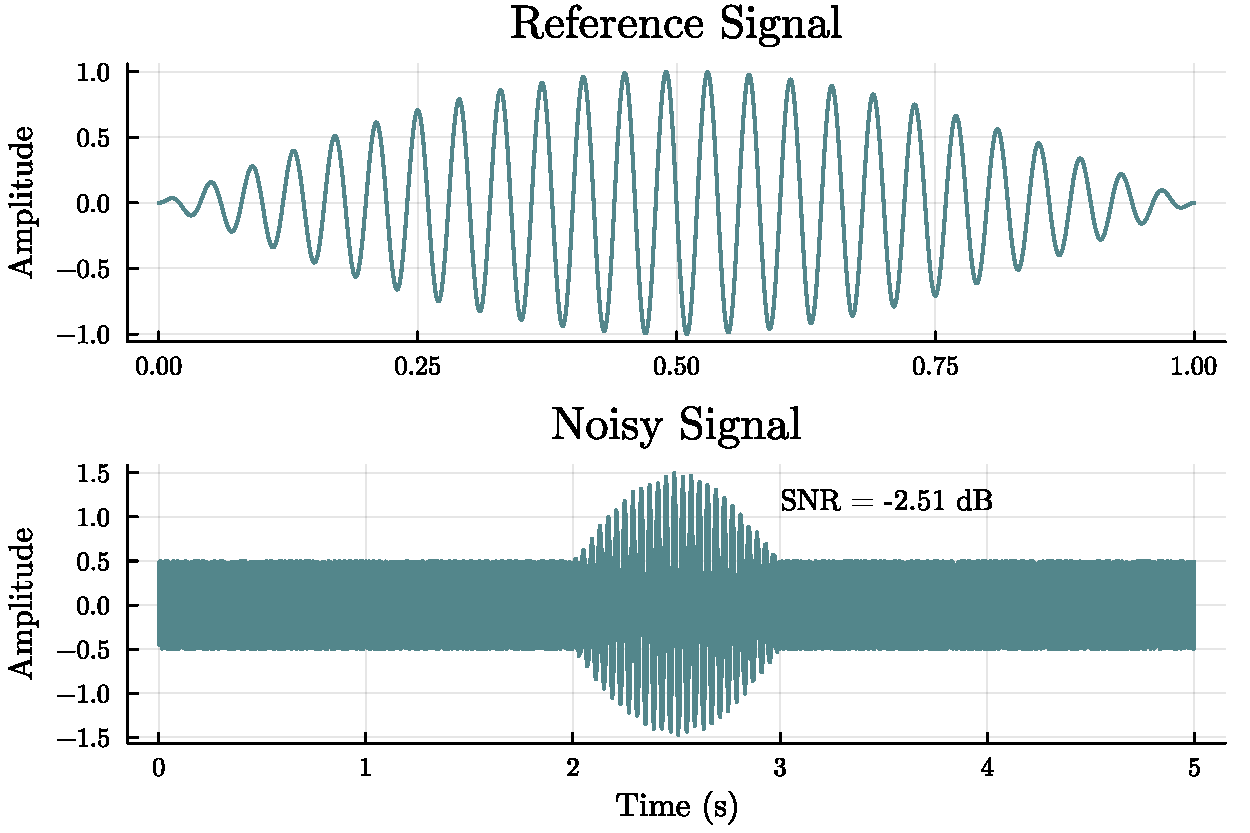
\includegraphics[width=\textwidth]{images/Background/Cross Correlation Reference and Data.pdf}
            \caption{Original signal and reference wave used for correlation operation}
            \hfill
            \label{fig: original data set and ref}
        \end{subfigure}
        \hfill
            \begin{subfigure}[c]{0.49\textwidth}
            \centering
            \captionsetup{width=0.75\textwidth}
            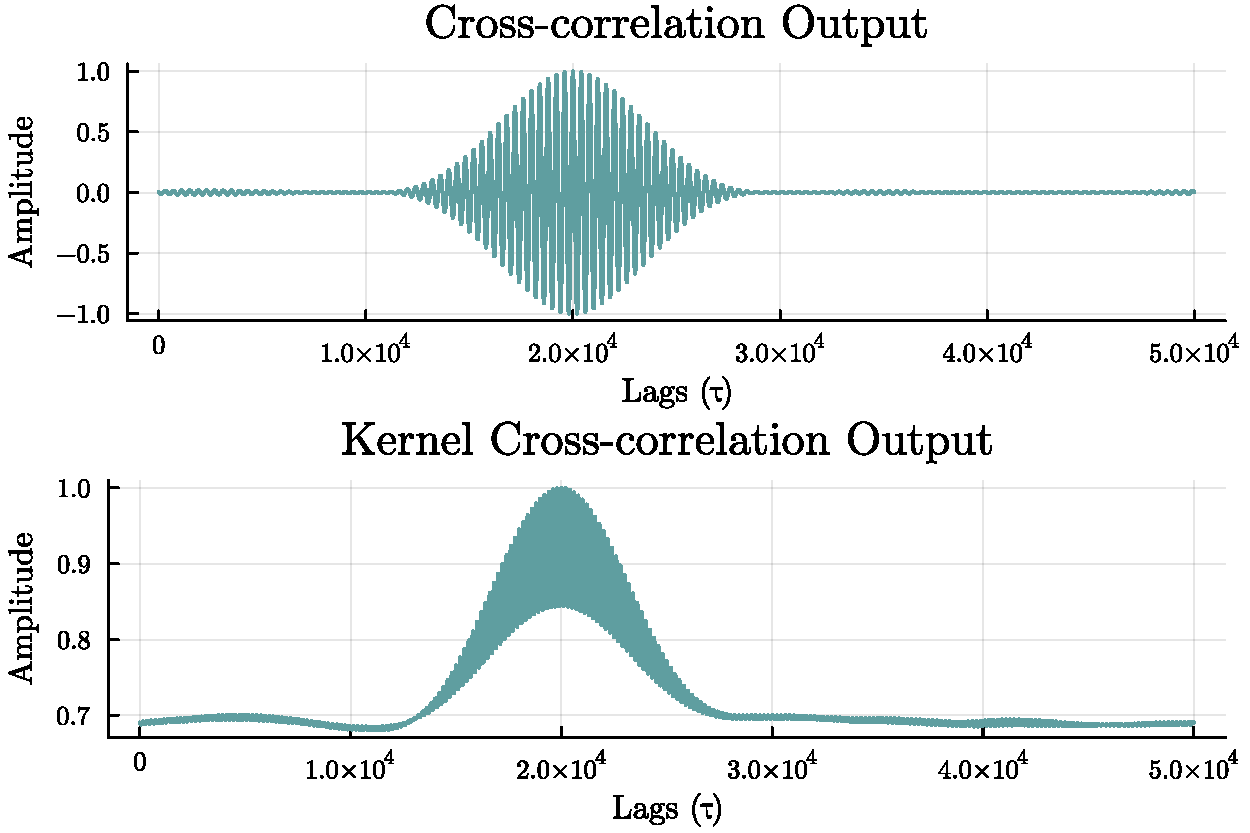
\includegraphics[width=\textwidth]{images/Formulation/Correlation Comparisons.pdf}
            \caption{Correlation output and kernel cross-correlation output}
            \hfill
            \label{fig: Correlation outputs}
        \end{subfigure}
        \hfill
        \caption{Comparison of a traditional cross-correlation to the kernelized version for the two data sets given in (a). The original signal contains a sine wavelet, beginning at 3 seconds, and additive white Gaussian noise. The SNR is calculated to be -7.33 dB.}
        \label{fig:Maps examples}
        \hfill
    \end{figure}

    The benefit of the frequency domain definition of the kernel cross-correlation is the ability to scale up the datasets $x$ and $y$ from a vector form $x,y \in \mathbb{R}^n$ into a matrix form $x,y \in \mathbb{R}^{m \times n}$. This flexibility allows for fast template matching in images as proposed by Wang et al. \cite{wang_kernel_2018}. The canonical, non-normalized version of the cross-correlation lacks the accuracy needed for template matching and therefore the normalized version proposed by Lewis \cite{lewis_fast_1995} is used as shown in figure \ref{fig:template match example}. The introduction of image kernel transformations and the mapping set $\hat{G}(z_p)$, greatly increases template matching accuracy in the non-normalized version of the correlation. Thus eliminating the need to compute the integral of the image and image power of the original image. Gaussians, which are commonly used to smooth images, can be easily programmed into the mapping set to reject noise and increase template matching accuracy. 

    \begin{figure} [h]
        \centering
        \begin{subfigure}[c]{0.49\textwidth}
            \centering
            \captionsetup{width=0.75\textwidth}
            \includegraphics[width=\textwidth]{images/Formulation/KCC_Gauss_Mapped_Output.jpg}
            \caption{The template matching correlation output yielded by kernel cross-correlator}
            \label{fig:KCC Template Output}
        \end{subfigure}
            \begin{subfigure}[c]{0.49\textwidth}
            \centering
            \captionsetup{width=0.75\textwidth}
            \includegraphics[width=\textwidth]{images/Formulation/Tulips Detected KCC.jpg}
            \caption{Original image with box placed where tulips are detected}
            \label{fig:KCC Template Matched}
        \end{subfigure}
        \hfill
        \caption{The kernel cross-correlation used in template matching for the same example photo as used in \ref{fig:template match example}. (a) Shows the correlation output yielded by the correlation algorithm when a cubic kernel and Gaussian mapping set are used. Multiple different reference images were used in the correlation calculations. (b) Shows the location of where the template matching placed the location of the flowers in the image.}
        \label{fig:KCC Used in Template Matching}
        \hfill
    \end{figure}

    \nomenclature{SSE}{Sum of Squared Errors}

    \subsection{Spectral Analysis}

    Much like the use of the classic correlation, the kernelized version of the cross-correlation can also be used to determine spectral content within a signal. This could provide use for power spectral analyses and frequency identification for signals with low SNR values. 

    Beginning with the autospectrum or power spectral density, it can be constructed via the frequency domain definition of the autospectrum. This allows a kernelized version of the PSD to be calculated using a combination of equations \ref{eq:PSD} and \ref{eq: KCF}. This yields the power spectral density of the kernel transformation of the data. 

    \begin{equation} \label{eq:KPSD}
        {S}_{xx}(\omega) = \hat{K}_t(x, x) \odot \hat{K}_t^*(x, x)
    \end{equation}

    The kernel function transformation rejects the noise within the data set, which in turn will allow for a clearer picture of the frequency content inside of a noisy data set. The kernelized version of the PSD is an effective way to measure the presence of stationary signals within data. Non-stationary signals that vary in frequency like a chirp can be detected, and will present as multiple frequencies or a frequency "bar". However, no temporal or phase information can accurately be discerned from the data because it returns a purely real output, therefore it is not ideal for analyzing non-stationary signals. 

    \begin{figure}[h]
        \centering
        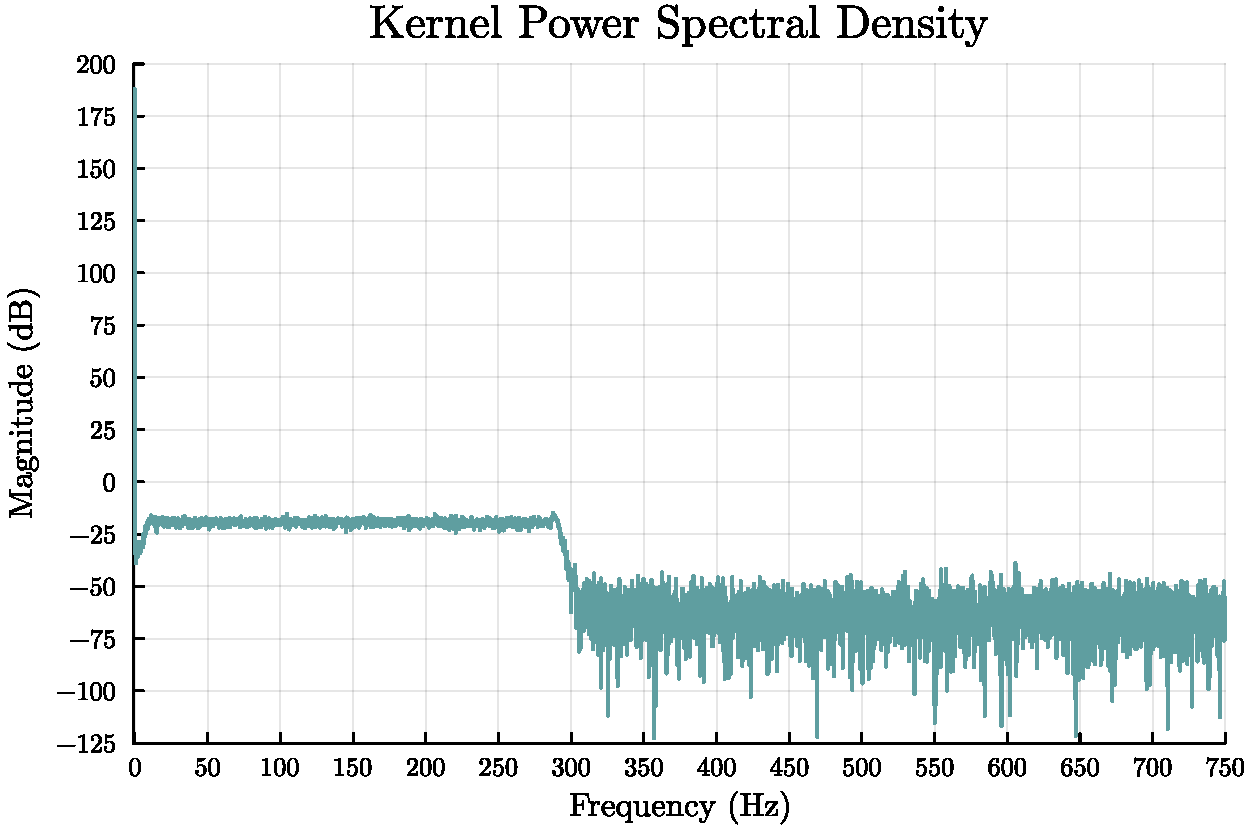
\includegraphics[scale = 0.5]{images/Formulation/KPSD example.pdf}
        \caption{The power spectral density using a Gaussian kernel of a chirp signal in noise having a linear frequency sweep from 10-300 Hz. The bar measuring -20dB raised above the noise indicates the dominant frequencies within the data set.}
        \label{fig:kpsd example}
    \end{figure}

    The kernelized version of the cross-spectrum follows a similar definition of the kernel power spectral density, and again would be a combination of equations \ref{eq:PSD} and \ref{eq: KCF}. 
    
    \begin{equation} \label{eq:KCSD}
        {S}_{xx}(\omega) = \hat{K}_t(x, x) \odot \hat{Y}^*(\omega)
    \end{equation}
    
    It is a further evolution that modifies the second term and uses the reference data set $y(t)$ that is used to check for specific frequency content. However unlike equation \ref{eq: KCF}, the use of a transformed reference is not desired. This ensures that the reference maintains the same frequency content and it is not changed by transformation. By checking for shared frequency content between two time-series, the kernel cross-spectral density can strongly indicate the presence of a signal within data. 

    \begin{figure}[h]
        \centering
        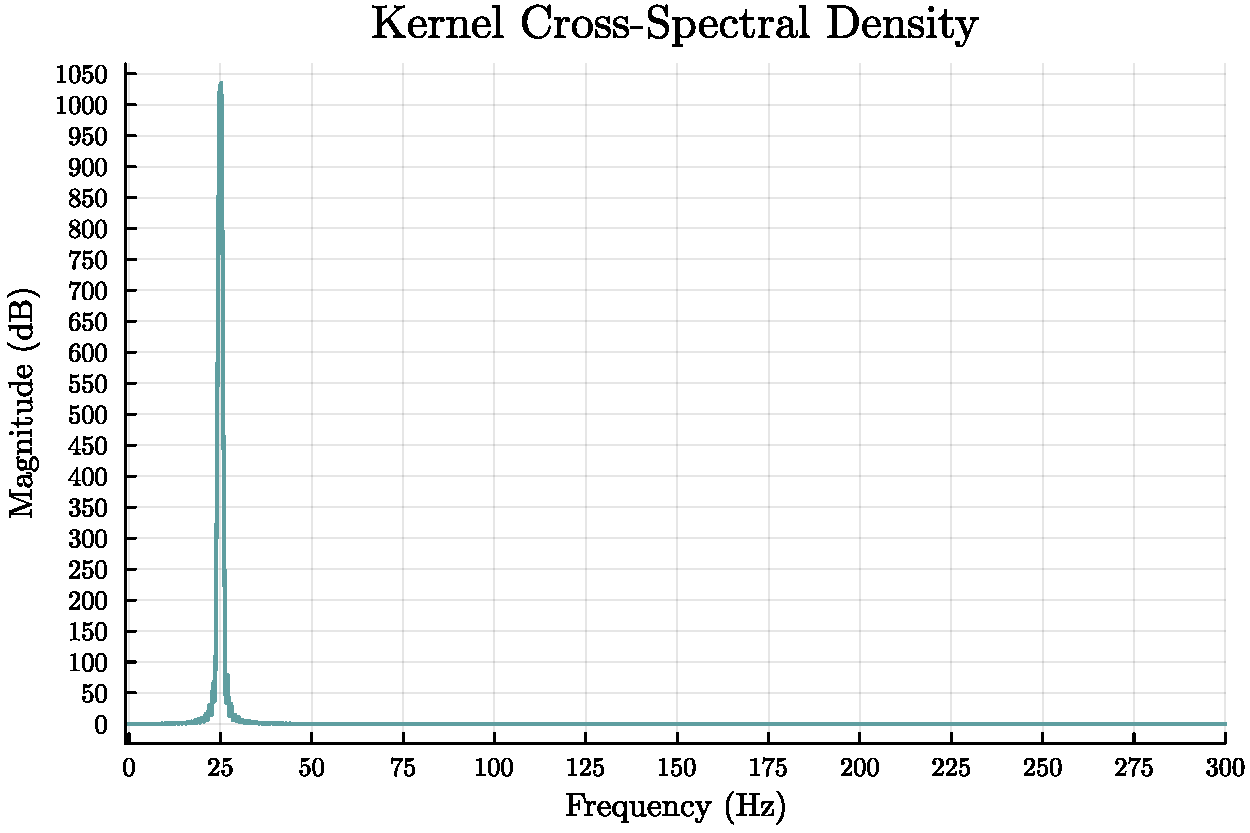
\includegraphics[scale = 0.5]{images/Formulation/KCSD example.pdf}
        \caption{The kernel cross-spectrum of the same chirp used in figure \ref*{fig:kpsd example} checked against the same wavelet shown in \ref{fig: original signal autocorr}, identical to the cross-spectrum in figure \ref{fig:CSD Example}. The spike appears at the shared frequencies between the two, which is 25 Hz. The kernel cross-spectrums peak appears larger than the classical form, however, unlike the classical form, there isn't the same frequency band from 10-300 Hz showing dominant frequencies in the noisy chirp data. The SNR for the noisy data was -2.5 dB}
        \label{fig:enter-label}
    \end{figure}